\documentclass{beamer}

\input{preamble.tex}
\usepackage{breqn} % Breaks lines

\usepackage{amsmath}
\usepackage{mathtools}

\usepackage{pdfpages} % \includepdf

\usepackage{listings} % R code
\usepackage{verbatim} % verbatim

% Video stuff
\usepackage{media9}

% packages for bibs and cites
\usepackage{natbib}
\usepackage{har2nat}
\newcommand{\possessivecite}[1]{\citeauthor{#1}'s \citeyearpar{#1}}
\usepackage{breakcites}
\usepackage{alltt}

% tikz
\usepackage{tikz}
\usepackage{pgfplots}
\usetikzlibrary{calc, positioning, decorations.pathreplacing, arrows.meta, intersections}
\pgfdeclarelayer{bg}
\pgfdeclarelayer{back}
\pgfdeclarelayer{fg}
\pgfsetlayers{bg,main,fg,back}
\usetikzlibrary{shapes,arrows}

% Setup math operators
\DeclareMathOperator{\E}{E} \DeclareMathOperator{\tr}{tr} \DeclareMathOperator{\se}{se} \DeclareMathOperator{\I}{I} \DeclareMathOperator{\sign}{sign} \DeclareMathOperator{\supp}{supp} \DeclareMathOperator{\plim}{plim}
\DeclareMathOperator*{\dlim}{\mathnormal{d}\mkern2mu-lim}
\newcommand\independent{\protect\mathpalette{\protect\independenT}{\perp}}
   \def\independenT#1#2{\mathrel{\rlap{$#1#2$}\mkern2mu{#1#2}}}
\newcommand*\colvec[1]{\begin{pmatrix}#1\end{pmatrix}}

\newcommand{\myurlshort}[2]{\href{#1}{\textcolor{gray}{\textsf{#2}}}}


\begin{document}

\imageframe{./lecture_includes/mixtape_ci_cover.png}


% ---- Content ----

\section{Introducing Regression Discontinuity Design}


\subsection{Basic background}



\begin{frame}{What is regression discontinuity?}

RDD is an extremely popular particular type of research design.  

\bigskip

Invented by Donald Campbell, educational psychologist, it went dormant for decades until around 1999 when I got ``rediscovered'' by Josh Angrist, Victor Lavy and Sandra Black

\bigskip

Often thought to be the most ``credible'' of the observational designs, even though it does not depend on randomization for identification

\end{frame}

\imageframe{./lecture_includes/currie_2.jpg}


\begin{frame}[plain]

	\begin{figure}
	\makebox[\textwidth][c]{\includegraphics[width=0.8\textwidth]{./lecture_includes/RDD_overtime.jpg}}%
	\end{figure}

\end{frame}

%\begin{frame}[plain]
%	\begin{center}
%	\textbf{Tell me what you think is happening}
%	\end{center}
	
%	\begin{figure}
%  \makebox[\textwidth][c]{\includegraphics[width=1.2\textwidth]{./lecture_includes/carpenter_aej.pdf}}%
%	\end{figure}
%\end{frame}



\begin{frame}{Regression discontinuity design}

	\begin{itemize}	
	\item We want to estimate some causal effect of a treatment on some outcome
	\item But we can't compare two groups (treated and not treated) because of the self selection (perfect doctor) which creates selection bias
	\item But what if treatment assignment was forced on units because the firm or agency uses a multi valued variable and splits the sample when units are above or below some threshold?
	\item RDD formalizes this setup and under some assumptions will identify causal effects
	\end{itemize}
\end{frame}

\begin{frame}{Classes of identification assumptions}


\begin{itemize}
\item \textbf{Independence assumption} -- largely associated with physical randomization, eliminates selection bias
	\begin{itemize}
	\item RCTs and A/B tests
	\item Matching and weighting (selection on observables)
	\item Instrumental variables
	\end{itemize}
\item \textbf{Restricting potential outcomes} -- largely associated with RDD, DiD and synthetic control
	\begin{itemize}
	\item Regression discontinuity design -- restricts $E[Y^0]$ and $E[Y^1]$ across some threshold
	\item Difference-in-differences -- restricts $E[Y^0 | D=1]$ to change over time in a restricted way\
	\item Synthetic control -- models $Y^0$ as a factor model
	\end{itemize}
\end{itemize}
	
\end{frame}

\begin{frame}{Breakout: RDD pictures}

 Each of the following 3 (but 4 slides) pictures is telling a story with distinct statistical objects

\bigskip

Help me understand the questions at the bottom of each picture by discussing what you think is happening


\end{frame}




\begin{frame}{RDD picture \# 1}
	
	\begin{figure}
  \makebox[\textwidth][c]{\includegraphics[width=0.75\textwidth]{./lecture_includes/alcohol_drinking1}}%
	\end{figure}

\textbf{Question}: What is age doing here? What's the story being told?

\end{frame}

	
	
\begin{frame}{RDD picture \# 2}
	
	\begin{figure}
  \makebox[\textwidth][c]{\includegraphics[width=0.75\textwidth]{./lecture_includes/alcohol_mortality}}%
	\end{figure}

\textbf{Question}:What do you think each dot represents? What do you think each line represents? What's the story being told?
	
	
\end{frame}

\begin{frame}{RDD picture \# 3}
	
	\begin{figure}
  \makebox[\textwidth][c]{\includegraphics[width=0.75\textwidth]{./lecture_includes/alcohol_mortality}}%
	\end{figure}

\textbf{Question}:Where is the treatment effect on the graph? Treatment effect \emph{of what}? Give a rough approximation of the treatment effect?
	
	
\end{frame}






\begin{frame}{Examples of RDD}

\begin{itemize}
\item Rather than cover examples at the end, I'd like to cover it at the front
\item I'll keep jargon to a minimum, and skip over identification issues
\item Hope is that this sparks some ideas for your own work
\end{itemize}

\end{frame}


\begin{frame}{Rounding to nearest star}

\begin{itemize}
\item Several interesting papers use a ``rounding to nearest star'' approach (\textbf{tons} of these papers, both in industry and social science applications)
	\begin{itemize}
	\item Michael Luca (2011) looks at restaurant revenue
	\item Anderson and Magruder (2011) look at wait times at restaurants, 
	\item Dell and Querubin (2018) look at bombing runs in Vietnam war
	\end{itemize}
\item Let's summarize these at a high level
\end{itemize}

\end{frame}

\begin{frame}{Example: Yelp and Tripadvisor}

\begin{itemize}
\item \textbf{Basic idea}: Customers review a firm which creates an average and continuous score, but for reasons related to customer expectations, platforms round the score to the nearest star or half star
\item \textbf{Research question}: Helps address effect selection bias related to firm quality and outcomes; estimates the effect of stars on outcomes
\item \textbf{Application}: Yelp and Tripadvisor data and application
\end{itemize}

\end{frame}

\begin{frame}{Stars and Restaurant Revenue}

\begin{itemize}

\item Michael Luca wants to know the effect of restaurant ``stars'' on restaurant revenue
\item Problem is, if you compare restaurants with different stars, it's almost certainly contaminated with selection bias$$E[Y^0|Star=4] \neq E[Y^0|Star=3]$$
\item That's because people \emph{give} stars to \emph{better} restaurants which likely would have had revenue even without the star (because they're great!  Word of mouth, etc.)
\end{itemize}

\end{frame}

\begin{frame}{Naive comparisons}
	
	\begin{figure}
  \makebox[\textwidth][c]{\includegraphics[width=0.5\textwidth]{./lecture_includes/luca_ols}}%
	\end{figure}

	
	
\end{frame}



\begin{frame}{Strategy: RDD}

\begin{itemize}

\item Luca's idea (and others) to address selection bias is to take advantage of a quirk on Yelp's website
\item Customers review the restaurants, which creates an average score, but Yelp only displays stars based on the score rounded to nearest half star
\item RDD will identify the LATE \emph{at} the point where firms' average score just barely tipped them over to the higher star

\end{itemize}

\end{frame}


\begin{frame}{Rounding to nearest star}
	
	\begin{figure}
  \makebox[\textwidth][c]{\includegraphics[width=0.75\textwidth]{./lecture_includes/luca_model}}%
	\end{figure}

	
	
\end{frame}



\begin{frame}{Data}

\begin{itemize}
\item \textbf{Yelp data}: Unclear how Luca got this.  Either he worked with them (possible) or he scraped the site (also possible). But this is where he gets stars and the continuous mean review
\item \textbf{Revenue data}:Washington Department of Revenue allows him to identify 3,582 unique restaurants at the time he got the data; 143 chains
\end{itemize}

\end{frame}

\begin{frame}{Estimation}

\begin{itemize}
\item \textbf{Pictures}:  I will focus on the pictures for now
\item \textbf{OLS regressions}: Luca accompanies his pictures with regression models \emph{of a particular specification}
\end{itemize}

\end{frame} 


\begin{frame}{Rounding to nearest star}
	
	\begin{figure}
  \makebox[\textwidth][c]{\includegraphics[width=0.7\textwidth]{./lecture_includes/luca_revenue}}%
	\end{figure}

\bigskip

\textbf{Discussion}: Approximately how much does an additional half-star change revenue? And what is Luca's evidence?
	
\end{frame}


\begin{frame}{Good Restaurants are Popular}

\begin{itemize}
\item Anderson and Magruder (2011) -- same idea. Higher rated stars have longer wait times
\item But we still don't know -- is it the star?  Or is the underlying quality?  Stars are based on unobserved quality
\item How will they separate selection bias from causality: Yelp average reviews, star rounding, merged wait times
\end{itemize}

\end{frame}

\begin{frame}{Data}

\begin{itemize}
\item \textbf{Context}: San Francisco (Luca had looked at Seattle which has lower rated restaurants)
\item \textbf{Scraped Yelp}: ``When clicking on an individual business, Yelp.com displays the entire history of reviews for that business.  We downloaded the history for each restaurant on Yelp.com and recorded the date of the review, the rating assigned (1-5), and the reviewer's unique user identifier. We then reconstructed the average rating and total number of reviews for each restaurant at every point in time.''
\item \textbf{Outcome}: Reservation availability data from ``large online reservation website'' which lists real-time reservation availability for hundreds of restaurants in SF then merged with Yelp data

\end{itemize}

\end{frame}

\begin{frame}{Wait times and star: pictures}
	
	\begin{figure}
  \makebox[\textwidth][c]{\includegraphics[width=0.35\textwidth]{./lecture_includes/yelp_waits}}%
	\end{figure}

	
\end{frame}


\begin{frame}{Wait times and star: OLS}
	
	\begin{figure}
  \makebox[\textwidth][c]{\includegraphics[width=0.7\textwidth]{./lecture_includes/yelp_ols_wait}}%
	\end{figure}
	
\end{frame}

\begin{frame}{Discussion}


\begin{enumerate}
\item  ``Explain to me like I'm 5'' your interpretation of their conclusions.
\item What parameter have they identified?
\end{enumerate}

\end{frame}







\subsection{Identification Basics}


\begin{frame}{Some RDD jargon terms}

\begin{itemize}
\item \textbf{Running variable}: a usually continuous score that some firm or agency uses to assign treatments to units
\item \textbf{Trends}: Not time trends; changing outcomes along the running variable (e.g., food gets better for restaurants with higher star ratings)
\item \textbf{Cutoff} or \textbf{threshold}: a particular value at a point on the running variable above which the firm or agency assigns treatments to unit
\item \textbf{Discontinuity} and/or \textbf{Jump}: Since we are \emph{estimating} breaks in the outcome right at the cutoff, and when that happens we say that there is a ``discontinuity''
\item \textbf{Regression}: Many of the models are simple difference in means, local regressions from OLS or global regressions from OLS
\end{itemize}

\end{frame}




	
\begin{frame}{Switching equation}

Recall our definitions around notation $Y$

\begin{enumerate}
\item Potential outcomes have superscripts, $Y^1_i$, $Y^0$. They refer to a person $i$ hypotheticals in worlds with or without treatment \emph{regardless if that happened}
\item One of these two is chosen when a treatment, $D_i$, is chosen according to the switching equation $$Y_i = DY^1_i + (1-D)Y^0_i$$
\item Observed outcomes have no superscripts, $Y_i$. They refer to a person $i$ observed outcome which is selected from one of their two potential outcomes (with binary treatments)
\end{enumerate}
\bigskip
The idea of a counterfactual is based on (1), not (2)

\end{frame}




\begin{frame}{Some common types of RDD}

		\begin{itemize}
		\item \textbf{Rounding}: Restaurants get ``stars'' (e.g., Michelin) and more revenue, but the ones that get more stars were probably better restaurants even without the star.  Yelp rounds to the nearest half star even though the underlying ``score'' is continuous.  The continuous score assigns stars
		\item \textbf{Close elections}: Majority voting, with a cutoff of 0.5, assigns different political parties into power
		\item \textbf{Algorithms}: Uber's surge pricing based on underlying demand measures 
		\item \textbf{Biology}: Age and drinking; Birthweight and ICU medical care
		\end{itemize}

\end{frame}

\begin{frame}{Data requirements}

Large sample sizes are characteristic features of the RDD

		\begin{itemize}
		\item If there are strong trends in the running variable, one typically needs a lot more data than if there weren't
		\item If the observations tend to be noisy, we need more data than if it was less noisy
		\item We need a lot of data bc we need significant mass at the running variable to reject the null
		\item Rewards people with access to firm level data since it can be large
		\end{itemize}
Might explain why the method never caught on until the 00's	


\end{frame}




\subsection{Sharp Design}

\begin{frame}{Sharp vs. Fuzzy RDD}
	
\begin{itemize}
\item There's two classes of RD designs:
	\begin{enumerate}
	\item \underline{Sharp RDD}: Treatment is a deterministic function of running variable, $X$. Example: Medicare benefits.  
	\item \underline{Fuzzy RDD}: Discontinuous ``jump'' in the \emph{probability} of treatment when $X>c_0$.  Cutoff is used as an instrumental variable for treatment.  Example: attending state flagship
	\end{enumerate}
\item Fuzzy is a type of IV strategy and requires explicit IV estimators like 2SLS; sharp is reduced form IV and doesn't require IV-like estimators -- we study it later with IV therefore
\end{itemize}	

\end{frame}	


\begin{frame}[plain]
\begin{figure}
\centering
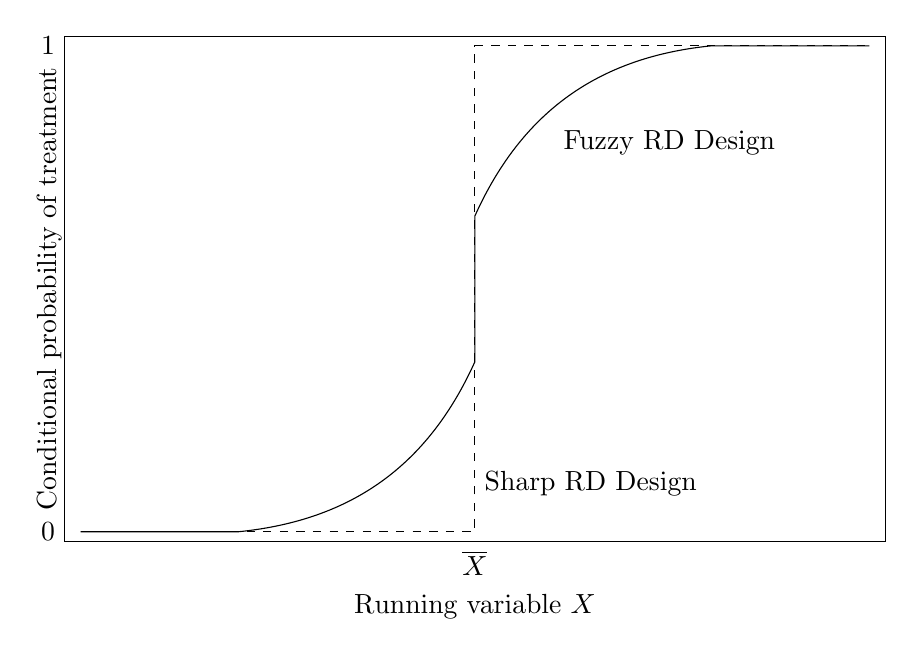
\begin{tikzpicture}
	\begin{axis}[
		xlabel={Running variable $X$},
		ylabel={Conditional probability of treatment},
		ylabel style={yshift=-0.5cm},
		ytick style={draw=none},
		xtick style={draw=none},
		width=12cm,
		height=8cm,
		xmin=-0.02,
		xmax=1.02,
		ymin=-0.02,
		ymax=1.02,
		xtick={0.5},
		xticklabel={$\overline{X}$},
		ytick={0,1}
	]
	
	\draw [dashed] (axis cs:0,0) -| (axis cs:0.5,1) -- (axis cs:1,1);
	\draw (axis cs:0,0) to 
				(axis cs:0.2,0) to 
				[bend right=30] (axis cs:0.5,0.35) to
				(axis cs:0.5,0.65) to
				[bend left=30] (axis cs:0.8,1) to
				(axis cs:1,1);
				
	\node [anchor=west] at (axis cs:0.5,0.1) {Sharp RD Design};
	\node [anchor=west] at (axis cs:0.6,0.8) {Fuzzy RD Design};
	
	\end{axis}
		
\end{tikzpicture}
\caption{Sharp (dashed) vs. Fuzzy (solid) RDD}
\end{figure}

	

\end{frame}

\begin{frame}{Some RDD issues}

\begin{itemize}
\item \textbf{Common support}: we don't have units in treatment and control along the running variable which makes comparisons across the running variable impossible
\item \textbf{Treatment effects}: we are estimating LATEs, like IV, because we are only estimating treatment effects \emph{at the cutoff} and that may not be informative of any other point on the running variable with extremely heterogeneity
\end{itemize}

\end{frame}

\begin{frame}{Some RDD issues}

\begin{itemize}
\item \textbf{Identification}: RDD does not requires the independence assumption for our estimators to ``work'', so what does it require?
\item \textbf{Extrapolation}: RDD uses regression and nonparametric methods by comparing units just below and above the cutoff to one another
\item \textbf{Variance vs bias}: Comparisons around the cutoff require large samples at that point, which will often require ``moving away'' from the cutoff and that re-introduces the selection bias we are concerned with
\end{itemize}

\end{frame}




\begin{frame}{Extrapolation, common support and functional form}

\begin{itemize}
\item Lacking common support, we must compare units ``around the cutoff'' (i.e., $X<c_0$ and $X\geq c_0$)
\item This requires ``extrapolation''; prediction beyond the support of the data (i.e., where treatment switches at cutoff)
\item But since you're predicting, modeling choices like \textbf{functional form} are key and that's a structural assumption
\end{itemize}

\end{frame}

\begin{frame}{Treatment assignment in the sharp RDD}

		\begin{block}{Deterministic treatment assignment (``sharp RDD'')}
		In Sharp RDD, treatment status is a deterministic and discontinuous function of a covariate, $X_i$:  $$D_i =\begin{cases} 1 \text{ if }& X_i\geq{c_0} \\ 0 \text{ if } & X_i < c_0  \end{cases}$$where $c_0$ is a known threshold or cutoff.  In other words, if you know the value of $X_i$ for a unit $i$, you know treatment assignment for unit $i$ with certainty.  
		\end{block}
	
\end{frame}	


\begin{frame}{Treatment effect definition and estimation}
	
	\begin{block}{Definition of treatment effect}
	The treatment effect parameter, $\delta$, is the discontinuity in the conditional expectation function:
		\begin{eqnarray*}
		\delta&=&lim_{X_i\rightarrow{c_0}}E[Y^1_i|X_i=c_0] - lim_{c_0\leftarrow{X_i}}E[Y^0_i | X_i=c_0] \\
			&=&lim_{X_i\rightarrow{c_0}}E[Y_i|X_i=c_0] - lim_{c_0\leftarrow{X_i}}E[Y_i | X_i=c_0]
		\end{eqnarray*}The sharp RDD estimation is interpreted as an average causal effect (LATE) of the treatment ($D$) at the discontinuity ($c_0$) $$\delta_{SRD}=E[Y^1_i - Y_i^0 | X_i=c_0]$$
	\end{block}
\end{frame}

\begin{frame}{Discussion}

In social policy, Medicare, age and age 65 are decent examples of a sharp RDD.

\bigskip

What's an example of running variables you've seen in your fields?  What's a treatment and cutoff?


\end{frame}
	





\subsection{Smoothness and Identification}



\begin{frame}{Smoothness vs Treatment Effect}
\begin{figure}
    \centering
    \includegraphics[width=5cm]{./lecture_includes/smoothness.png}
    \qquad
    \includegraphics[width=5cm]{./lecture_includes/LATE_RDD.png}
    \caption{Smoothness of potential outcomes (left) vs estimation of LATE (right)}
\end{figure}

\textbf{Discussion}: Why is the left picture different from the right picture? Where did the two lines go?



\end{frame}




\begin{frame}{Smoothness as the identifying assumption}
	
	\begin{block}{Smoothness of conditional expected potential outcome functions through the cutoff}
	$E[Y_i^0 | X=c_0]$ and $E[Y_i^1 | X=c_0]$ are continuous (smooth) in $X$ at $c_0$. 
	\end{block}
	
	\begin{itemize}
	\item If population average \emph{potential outcomes}, $E[Y^1]$ and $E[Y^0]$, are smooth functions of $X$ across the cutoff, $c_0$, then expected potential average outcomes \emph{won't} jump at $c_0$. 
	\item Implies that the confounders are also evolving smoothly across the cutoff 
	\end{itemize}
	
\end{frame}


\begin{frame}{Smoothness is untestable}
	

	\begin{itemize}
	\item Smoothness lets us justify extrapolation across $c_0$ 
	\item Average causal effect is defined \emph{at the cutoff}, but estimation uses data \emph{around the cutoff} 
	\item IOW, identification and estimation are not the same thing -- smoothness is what gives our estimates a causal interpretation
	\end{itemize}
	
\end{frame}


\begin{frame}{Potential and observable outcomes}

	\begin{itemize}
	\item \textbf{Question}: Why doesn't a discontinuity in $Y$ at $X=c_0$ imply smoothness is violated?
	\item \textbf{Hint}: Recall how we moved between potential and observable outcomes using the switching equation in ``perfect doctor'': $$Y_i = DY^1_i + (1-D)Y^0_i$$
	\item \textbf{Answer}: We \emph{observe} $E[Y_i|X_i]$ but smoothness is about the performance of expected potential outcome functions, $E[Y^0_i|X_i]$ or $E[Y^1_i|X_i]$
	\end{itemize}

\end{frame}

\section{Estimation}

\subsection{Global and Local Regressions}



\begin{frame}{Estimation with extrapolation}
	
	\begin{itemize}
	\item We use \emph{extrapolation} to estimate average treatment effects with the sharp RDD which is unbiased under \emph{smoothness}
	\item Our statistical models predict expected conditional \emph{counterfactuals} using data on \emph{the other side of the cutoff}
	\item Keep in mind though: the actual aggregate causal effect is $Y^1_i - Y^0_i$ at any point on $X_i$ -- not across $X=c_0$
	
	\end{itemize}

\end{frame}


\begin{frame}{Re-centering the running variable}
	
	\begin{itemize}
	\item Assume a linear function $$Y_i = \alpha + \beta(X_i) + \delta D_i + \varepsilon_i$$
	\item People will often ``re-center'' by subtracting $c_0$ from $X_i$:$$Y_i=\alpha + \beta(X_i-c_0) + \delta D_i +\varepsilon_i$$
	\item This doesn't change the interpretation of the treatment effect; just the intercept.
	\end{itemize}

\end{frame}



\begin{frame}{Re-centering the running variable}

\begin{itemize}
	\item Example: Medicare and age 65.  Center the running variable (age) by subtracting 65 from age:
		\begin{eqnarray*}
		Y &=& \beta_0 + \beta_1(Age) + \beta_2 Edu + \varepsilon \\
		&=& \beta_0 + \beta_1(Age-65) + \beta_2 Edu + \varepsilon\\
		&=& \beta_0 + \beta_1 Age - \beta_1 65 + \beta_2 Edu+ \varepsilon \\
		&=& \alpha + \beta_1 Age + \beta_2 Edu+ \varepsilon
		\end{eqnarray*}where $\alpha=\beta_0 - \beta_1 65$.  
		\item All other coefficients, notice, have the same interpretation, except for the intercept.
\end{itemize}

\end{frame}


\begin{frame}{Smooth but nonlinear conditional expected potential outcome functions}
	
	\begin{itemize}
	\item Smoothness is an assumption about the behavior of the conditional expected potential outcomes as we move across the running variable and through the cutoff
	\item Does not imply \emph{linear} evolution of expected potential outcomes though
	\item What if the trend relation $E[Y_i^0 | X_i]$ does not jump at $c_0$ but rather is simply nonlinear?  You could get spurious results
	\end{itemize}

\end{frame}


\begin{frame}{Approximate the functional form}

Two ways to estimate the treatment effect at $X=c_0$

\bigskip

		\begin{enumerate}
		\item Use global and local regressions with $f(X_i)$ equalling a $p^{th}$ order polynomial 
		\begin{eqnarray*}
		Y_i&=&\alpha +\delta{D_i}  +  \beta_1x_i + \beta_2x_i^2 + \dots + \beta_px_i^p + \eta_i
		\end{eqnarray*}
		\item Nonparametric kernel methods
		\end{enumerate}
\end{frame}

\begin{frame}{Potential outcomes and nonlinear running variable}
	
	\begin{itemize}
	\item We can generalize the function, $f(x_i)$, by allowing it to differ on both sides of the cutoff by including them both individually and interacting them with $D_i$.  
	\item In that case we have:
		\begin{eqnarray*}
		E[Y_i^0 | X_i] &=& \alpha + \beta_{01}\tilde{X}_i + \beta_{02}\tilde{X}_i^2 + \dots + \beta_{0p}\tilde{X}_i^p \\
		E[Y_i^1 | X_i] &=& \alpha + \delta + \beta_{11}\tilde{X}_i + \beta_{12}\tilde{X}_i^2 + \dots + \beta_{1p}\tilde{X}_i^p
		\end{eqnarray*}where $\tilde{X}_i$ is the centered running variable (i.e., $X_i - c_0$). 
	\item Notice the treatment effect in the second line, and the intrinsic ATE when comparing the two equations, $E[Y_i^0 - Y_i^1 | X_i]$	
	\end{itemize}
\end{frame}


\begin{frame}{Interact running variable with treatment}

\begin{itemize}
		\item Re-centering at $c_0$ ensures that the treatment effect at $X_i=c_0$ is the coefficient on $D_i$ in a regression model with interaction terms
		\item Interactions of treatment with running variable terms, $D \times X$, where $X$ has be re-centered allows for the ``two line'' pictures we've been looking at
\end{itemize}

\end{frame}



\begin{frame}{Regression equation}

\begin{itemize}
	\item Regression model you estimate is:
		\begin{eqnarray*}
		Y_i &=& \alpha + \beta_{01}\tilde{x}_i + \beta_{02}\tilde{x}_i^2 + \dots + \beta_{0p}\tilde{x}_i^p \\
		& & + \delta{D}_i + \beta_1^*D_i\tilde{x}_i + \beta_2^*D_i\tilde{x}_i^2 + \dots + \beta_p^*D_i\tilde{x}_i^p + \varepsilon_i 
		\end{eqnarray*}where $\beta^*_1 = \beta_{11} - \beta_{01}$, $\beta_2^* = \beta_{21} - \beta_{21}$ and $\beta_p^*=\beta_{1p}-\beta_{0p}$
	\item Notice the interactions of $D$ with the re-centered running variables -- they model the dynamics in the running variable above and below the cutoff
	\item Look closely at how the beta terms aren't the same for $D=0$ as they are for $D=1$ (which corresponds to below and above the cutoff)
	\item But the parameter of interest, the treatment effect, is the coefficient at $c_0$ or $\widehat{\delta}$
\end{itemize}

\end{frame}


\begin{frame}{Estimation without and with specifying nonlinear running variable}
\begin{figure}
    \centering
    \includegraphics[width=5cm]{./lecture_includes/linear_estimation.png}
    \qquad
    \includegraphics[width=5cm]{./lecture_includes/nonlinear_estimation.png}
    \caption{Spurious treatment effects with linear specification (left) versus 3rd order polynomial (right)}
\end{figure}

\textbf{Look close}: See how the lines don't touch on the left, but they do on the right?  

\end{frame}



\begin{frame}{Sharp RDD: Nonlinear Case}
	
	\begin{itemize}
	\item Suppose the nonlinear relationship is $E[Y_i^0 | X_i]=f(X_i)$ for some reasonably smooth function $f(X_i)$ (e.g., quadratic in $X$) 
	\item In that case we'd fit the regression model:$$Y_i=f(X_i) + \delta{D_i} + \eta_i$$
	\item But what is this $f(X_i)$? It models the counterfactual values of $Y^0$ and since we are extrapolating, we need an estimator that we think is extrapolating correctly
	\item There are 2 common ways of approximating $f(X_i)$	
	\end{itemize}
\end{frame}

\begin{frame}{OLS estimation with 3rd order polynomial}
	
	\begin{figure}
  \makebox[\textwidth][c]{\includegraphics[width=0.75\textwidth]{./lecture_includes/OLS_output.png}}%
	\end{figure}

	
\end{frame}

\begin{frame}{Comment about higher order polynomials}

\begin{itemize}
\item Very common to see polynomials introduced to model nonlinearities in potential outcomes
\item But higher order polynomials can have overfitting problems leading to poor prediction beyond the cutoff 
\item Gelman and Imbens (2018) caution against overfitting on these global regressions (i.e., quadratics) 
\end{itemize}

\end{frame}


\subsection{Nonparametric estimation}

\begin{frame}{Some new terms}

\begin{itemize}

\item \textbf{Kernels} make a window and give you the shape of the window (e.g., triangular kernels weight the observations differently within the window)
\item \textbf{Bandwidth} is the ``length'' of the window (small ones are tiny windows, bigger ones, bigger windows -- think of a histogram)
\item \textbf{Bins} are about the interval itself (a partition)

\end{itemize}

\end{frame}




\begin{frame}{Local linear nonparametric regressions}

\begin{itemize}
\item Least squares approaches models the counterfactual using functional forms which is parametric, but it can have poor predictive properties on counterfactuals above/below the cutoff
\item Another way of approximating the running variable flexibly $f(X_i)$ is to use a nonparametric kernel 
\item Hahn, Todd and Van der Klaauw (2001) proposed ``local linear nonparametric regressions'' which is weighted least squares for a given bandwidth $h$ and weights that vary by distance to the cutoff
\end{itemize}

\end{frame}



\begin{frame}{Local linear nonparametric regressions}
	
	\begin{itemize}
	\item Local linear nonparametric regression substantially reduces the bias
	\item Think of it as a weighted regression restricted to a window -- kernel provides the weights to that regression.  
	\item It's like a histogram (which weights each observation the same), but it's a regression with polynomial terms and the option for other weights than just uniform
	\end{itemize}
	
\end{frame}


\begin{frame}{Choices you have to make}

\begin{enumerate}
\item Choose the bandwidth $h$
\item Choose the kernel $K(\cdot)$
\item Choose the polynomial ordering $p$
\end{enumerate}
\bigskip
We have a broad set of writings and suggestions around each of these things, and the issues around choices is always subjective researcher bias, uncertainty and various forms of bias

\end{frame}



\begin{frame}{Local polynomial estimation steps}

\begin{enumerate}
\item Choose a polynomial order $p$ and a kernel function $K(\cdot)$
\item Choose a bandwidth $h$
\item For observations above the cutoff, fit a WLS regression of $Y$ on a constant and re-centered running variable terms with $p$ polynomial terms and weight $K(\frac{X_i-c}{h})$ for each observation which is an estimate of the point$\mu_+=E[Y_i^1|X_i=c]$:$$\widehat{\mu}_+:\widehat{Y}_i=\widehat{\mu}_+ + \widehat{\mu}_{+,1}(X_i-c)+\widehat{\mu}_{+,1}(X_i-c)^2 + \dots + \widehat{\mu}_{+,p}(X_i-c)^p$$
\item Repeat step 3 below the cutoff $\mu_-=E[Y_i^1|X_i=c]$:$$\widehat{\mu}_-:\widehat{Y}_i=\widehat{\mu}_- +. \widehat{\mu}_{-,1}(X_i-c)+\widehat{\mu}_{-,1}(X_i-c)^2 + \dots + \widehat{\mu}_{-,p}(X_i-c)^p$$
\item Calculate the sharp RD point estimate as $\widehat{\delta}=\widehat{\mu}_+ - \widehat{\mu}_-$
\end{enumerate}

\end{frame}


\begin{frame}{Animation of a local linear regression}

\url{https://twitter.com/page_eco/status/958687180104245248}

\end{frame}


\begin{frame}{Boundary problems}
	
		\begin{figure}
		\includegraphics[scale=1.2]{./lecture_includes/kernel_1.pdf}
		\end{figure}

``True'' effect at cutoff is $AB$, but in this histogram of width $h$, we estimate $A'B'$ because of trends in the running variable; what can we do?

	
\end{frame}


\begin{frame}{Local regressions with kernels}

		\begin{figure}
		\includegraphics[scale=0.24]{./lecture_includes/cattaneo_local}
		\caption{From Cattaneo, et al. (2019)}
		\end{figure}

\end{frame}

\begin{frame}{Estimation with kernels}

The kernel function $K(\cdot)$ assigns non-negative weights to each re-centered observation based on the distance between each observation's running variable score $X_i$ and the cutoff $c$ and there are different kinds of kernel weights you can choose

\end{frame}

\begin{frame}{Types of kernels}

\begin{itemize}
	\item \textbf{Rectangular} uniform weights equivalent to $E[Y]$ at a given bin on $X$
	\item \textbf{Triangular} give more importance to observations close to the center
\end{itemize}
\end{frame}

\begin{frame}{Estimation with kernels}


\begin{itemize}
\item Cattaneo, et al. (2019) recommend using the triangular kernel because when you use it with a bandwidth that optimizes mean squared error, you can get a point estimate that is optimal. 
\item Triangular kernels assign zero weight to all observations outside bandwidth $h$ interval and positive weights within it
\item Weights are maximized at the cutoff and decline symmetrically and linearly as the value of the running variable gets further away
\end{itemize}

\end{frame}

\begin{frame}

		\begin{figure}
		\includegraphics[scale=0.4]{./lecture_includes/cattaneo_kernels}
		\caption{From Cattaneo, et al. (2019)}
		\end{figure}

\end{frame}

\begin{frame}{Polynomial order}

\begin{itemize}
\item Simple difference in means (i.e., $p$ order of zero) is like a histogram with uniform weights
\item Suffers from what is called the ``boundary problem'' -- the estimation of the true expected potential outcomes at the cutoff is biased with trends in the running variable
\item But even after choosing kernel weights, we aren't done as then there is the business of choosing polynomial order
\end{itemize}

\end{frame}



\begin{frame}{Polynomial terms}

\begin{itemize}
\item Two conceptual issues to keep in mind
	\begin{enumerate}
	\item No polynomials has boundary problems, but
	\item Higher order polynomials, though, suffer from severe overfitting problems
	\end{enumerate}
\item Local linear RD is the preferred method, but this is where we end up in the world of choosing the bandwidths, $h$, because that controls the width (and thus selects the units) of the neighborhood around the cutoff that will be used to fit the model
\end{itemize}

\end{frame}


\begin{frame}

		\begin{figure}
		\includegraphics[scale=0.27]{./lecture_includes/cattaneo_bandwidth}
		\caption{From Cattaneo, et al. (2019)}
		\end{figure}

\end{frame}




\begin{frame}{Bias and variance}

\begin{itemize}
\item \textbf{Bias term}
	\begin{itemize}
	\item When we approximate the unknown functions with $p$, $h$ and $K(\cdot)$, there's some approximation error because we do now actually know the true function
	\item Think about the earlier picture -- when we used the larger bandwidth and $p$ of zero, we came up short. Why? Because of the curvature of the functions we were approximating
	\end{itemize}
\item \textbf{Variance term}
	\begin{itemize}
	\item Variance depends on sample size and bandwidth $h$
	\item As number of observations near the cutoff falls, the contribution of the variance term to MSE grows and vice versa
	\item Variability of the the point estimator depends therefore on density at the cutoff (which gets back to why RD tends to be data intensive in the first place)
	\end{itemize}
\end{itemize}

\end{frame}

\begin{frame}{Optimal Bandwidths}

\begin{itemize}
\item Most approaches have some balancing act between bias and variance that they're trying to address
\item Minimizing the MSE of the local estimator, $\widehat{\delta}$, given a choice of $p$ and $K(\cdot)$ has become the most popular since MSE is the sum of squared bias and variance $$MSE(\widehat{\delta}) = Bias^2(\widehat{\delta}) + Variance^(\widehat{\delta})$$
\item If you choose to minimize MSE, you are choosing $h$ -- hence ``optimal bandwidths'' $$min_{h>0} \bigg (h^{2(p+1)}B^2+\frac{1}{nh}V \bigg )$$
\end{itemize}

\end{frame}

\begin{frame}{Optimal Bandwidths}

\begin{itemize}
\item Solution to that minimization problem is $h_{MSE}$ and is the MSE-optimal bandwidth choice$$h_{MSE} = \bigg ( \frac{V}{2(p+1)}B^2 \bigg )^{\frac{1}{(2p+3)}}n^{-1/(2p+3)}$$which directly addresses the bias-variance trade-off
\item Optimal bandwidths that minimize MSE are proportional to that last term and therefore MSE-optimal bandwidths increase with $V$ (more observations) and decrease with $B$ (less observations)
\item Hence why optimal bandwidths are ``data driven'' and automated which takes away some of the subjective decisions researchers must make
\end{itemize}

\end{frame}


\begin{frame}{Implementation with software}

\begin{itemize}
\item You have choices for implementing this -- manually (see Cattaneo, et al. (2019) section 4.2.4, or with packages like \texttt{rdrobust} 
\item Very flexible -- choose kernels (e.g., triangular), choose polynomials, choose number of bandwidths $h$
\item But remember choosing $h$ is not advisable bc of what we just said, so there is a separate package called \texttt{rdbwselect} which selects the MSE-optimal bandwidth for the local estimator (but you still choose $p$ and $K(\cdot)$)
\end{itemize}

\end{frame}

\begin{frame}{Implementation with software}

\begin{itemize}
\item Tons of options with \texttt{rdbwselect} -- different kernels, even different bandwidths left and right of the cutoff
\item Once you use it, you can pass it on to \texttt{rdrobust} in a second stage, or
\item Just use \texttt{bwselect} within the syntax of \texttt{rdrobust} itself (we will review this with our Hansen exercise later)
\item All of this can be incorporated into plotting too with \texttt{rdplot}
\end{itemize}

\end{frame}


\begin{frame}{Inference}

\begin{itemize}
\item Asymptotic 95\% confidence intervals for an RD point estimator will be too small if they ignore the bias and variance terms$$CI=\bigg [ ( \widehat{\delta} - B) \pm 1.96 \cdot \sqrt{V} \bigg ]$$
\item Bias term arises because the local polynomial approach is a non-parametric approximation of the unknown potential outcome regression functions
\item So different strategies are used to address this 
\end{itemize}

\end{frame}

\begin{frame}{Corrections}
\begin{itemize}
\item \textbf{Conventional} confidence intervals assume that the polynomial gave an exact approximation of the potential outcomes, but as this can't be verified, it isn't considered credible $$CI_{us}=\bigg [ \widehat{\delta}  \pm 1.96 \cdot \sqrt{V} \bigg ]$$
\item If the approximation error is non-trivial, inference based on the conventional approach will be incorrect, over-rejection of the null of zero treatment effects
\item Cattaneo, et al. (2019) strongly discourage you from using this
\end{itemize}

\end{frame}


\begin{frame}{Standard bias correction confidence intervals}

\begin{itemize}
\item \textbf{Bias correction} confidence intervals adjust for bias by estimating the bias term $B$ with an estimator $\widehat{B}$  $$CI_{bc}=\bigg [ ( \widehat{\delta} - \widehat{B} ) \pm 1.96 \cdot \sqrt{V} \bigg ]$$
\item Bias term, as we said earlier in the MSE-optimal slides, depends on trends in the running variable for that unknown potential outcome function and whether that's captured by the polynomials you chose
\item But it can have poor performance in applications because the bias estimation step isn't incorporated in the variance term which can introduce coverage distortions in practice
\end{itemize}

\end{frame}


\begin{frame}{Robust bias correction confidence intervals}

\begin{itemize}
\item \textbf{Robust bias correction} confidence intervals are based on the bias correction procedure. which estimated the bias term with $\widehat{B}$ and includes a new asymptotic variance that incorporates the bias correction step  $$CI_{rbc}=\bigg [ ( \widehat{\delta} - \widehat{B} ) \pm 1.96 \cdot \sqrt{V_{bc}} \bigg ]$$
\item Because this new variance term incorporates the extra variability from that first bias estimation step, it's larger for the same bandwidth
\end{itemize}
\end{frame}


\begin{frame}{Different confidence intervals}


\begin{table}[htbp]\centering
\caption{Local polynomial confidence intervals (from Cattaneo, et al. (2019)}
\centering
\begin{tabular}{l*{2}{c}}
\toprule
\multicolumn{1}{l}{\textbf{}}&
\multicolumn{1}{c}{\textbf{Centered at}}&
\multicolumn{1}{c}{\textbf{Standard error}}\\
\midrule
Conventional: $CI_{us}$	& $\widehat{\delta}$	& $\sqrt{\widehat{V}}$ \\
Bias-corrected: $CI_{bc}$	& $\widehat{\delta} - \widehat{B}$	& $\sqrt{\widehat{V}}$ \\
Robust bias-corrected: $CI_{rbc}$	& $\widehat{\delta} - \widehat{B}$	& $\sqrt{\widehat{V_{bc}}}$ \\
\bottomrule
\end{tabular}
\end{table}

\end{frame}



\begin{frame}{Inference -- clustering and honesty}

\begin{itemize}
\item Historically, people would cluster standard errors along the running variable (going back to early work by Lee), but recent work warns against this
\item Koles\'ar and Rothe (2018) provide extensive theoretical and simulation-based evidence that clustering on the running variable has high over-rejection problems
\item Propose two alternative confidence intervals that achieve correct coverage in large samples -- called ``honest'' -- which is available in R (\texttt{RDHonest}) at \url{https://github.com/kolesarm/RDHonest}
\end{itemize}

\end{frame}

\subsection{Testing for violations}

\begin{frame}{Evaluating violations of smoothness}

\begin{itemize}
\item Smoothness isn't \emph{directly} verifiable because it involves counterfactuals for each unit along $X_i$ which don't exist bc of switching equation
\item Doesn't stop us!  People tend to use various ingenious deductions involving ``placebos''
\item People tend to want at least indirect evidence for smoothness since we don't have ``the science of physical randomization'' to ensure smoothness holds in our data
\end{itemize}

\end{frame}


\begin{frame}{Main Challenges}

Classify your concern regarding smoothness violations into two categories:
\begin{itemize}
\item Manipulation on the running variable 
\item Endogeneity of the cutoff
\end{itemize}Most robustness is aimed at building credibility around these, 

\end{frame}




\begin{frame}{Manipulation of your running variable score}
	
	\begin{itemize}
	\item Treatment is not as good as randomly assigned around the cutoff, $c_0$, when agents are able to manipulate their running variable scores.  This happens when:
		\begin{enumerate}
		\item the assignment rule is known in advance
		\item agents are interested in adjusting
		\item agents have time to adjust
		\item administrative quirks like nonrandom heaping along the running variable
		\end{enumerate}
	\item In other words, we are looking for evidence of people choosing their value of $X_i$ so as to get just barely get into the treatment
	\item \textbf{Example} an unusual bunching of reviews at the stars ``just below'' the cutoff on Yelp
	\end{itemize}
\end{frame}



\begin{frame}{Manipulation might violation smoothness}
	
	\begin{block}{Manipulation of the running variable}
Assume a desirable treatment, $D$, and an assignment rule $X\geq{c_0}$.  If individuals sort into $D$ by choosing $X$ such that $X\geq{c_0}$, then we say individuals are manipulating the running variable. 
	\end{block}
Also can be called ``sorting on the running variable'' -- same thing.

\bigskip

If the individuals who manipulated their score had different potential outcomes, it could create a gap even though it's just sorting

\end{frame}

\begin{frame}{Manipulation is testable}

Finally -- a testable prediction

\bigskip

	\begin{itemize}
		\item Noom, weight loss app, wants to keep people using the app
		\item When number of skipped logging of meals and weighing exceeds some threshold, a coach privately texts them
		\item We want to know the effect of coaches on retention
	\end{itemize}
			
\end{frame}

\begin{frame}{Manipulation along the running variable}

\begin{itemize}
	\item Manipulation may occur if:
		\begin{enumerate}
		\item Users can choose logging of meals and/or weighing (yes)
		\item Know about the cutoff score (probably not)
		\item Have enough time to change their behavior (yes)
		\end{enumerate}
	\item If all three, then we will tend to see ``bunching'' of people not logging around the cutoff
	\item Justin McCrary (2008 article) thought of this and suggested a ``density test'' to see if you could reject a null of smooth density at the cutoff 
\end{itemize}

\end{frame}


\begin{frame}{McCrary Density Test}

	\begin{itemize}
	\item Assumes a null where the \emph{density} is continuous at the cutoff point 
	\item Under the alternative hypothesis, the density increases at the cutoff as people sort onto the desirable side of the cutoff
	\item This is oftentimes visualized with confidence intervals illustrating the effect of the discontinuity on density - you need no jump to pass this test
	\item Not perfect, but pretty ingenious and is based on rational choice when you think about it
	\end{itemize}

\end{frame}

\begin{frame}{Steps for a density test in RDD}

		\begin{enumerate}
		\item Count observations for a chosen bin (needs multiple units in other words per bin)
		\item Estimate your nonlinear OLS model with quadratics in the running variable on the \emph{counts}
		\item Do you reject the null at the cutoff?
		\end{enumerate}There are updates to McCrary (2008) using other density tests but this is the basic idea
\end{frame}




\begin{frame}{Simulations of density tests}

	\begin{figure}
	\includegraphics[scale=0.75]{./lecture_includes/mccrary_density_test.pdf}
	\caption{\scriptsize From McCrary (2008). Left shows failing to reject.  Right shows rejection of the null.}
	\end{figure}

\end{frame}

\begin{frame}{Yelp density tests}
\begin{figure}
    \includegraphics[scale=0.35]{./lecture_includes/yelp_density}
    \caption{Number of observations (density) around the Yelp discontinuity}
\end{figure}


\end{frame}



\begin{frame}{Does NICU save premature babies' lives?}

\begin{itemize}
\item What is the causal effect of heightened medical care for premature babies on infant mortality?  
\item Babies in NICU have lower mortality even if they weren't in the NICU
\item Answer: use 1500 grams as the cutoff and large administrative data from hospitals
\end{itemize}

\end{frame}


\begin{frame}{Heaping problem}


\begin{figure}[htb]
\centering	\includegraphics[scale=0.08]{./lecture_includes/heaping.jpg}%.jpg}
\caption{Huge number of babies born with birth weights (grams) at non-random spaced intervals}
\end{figure}

\end{frame}



\begin{frame}{Why heaping at birth?}

\begin{itemize}
\item \textbf{H1}: Babies naturally born every 100 grams.  Unlikely. Babies can't choose their birthweight, nor can parents. Seems more likely births are uniformly distributed around some arbitrary cutoff
\item \textbf{H2}: Someone is rounding \emph{the running variable itself}
	\begin{itemize}
	\item Maybe some scales in some hospitals are less sophisticated
	\item Maybe rounding practices are more common in some types of hospitals than others
	\item Maybe parents and staff push for rounding to get favorable treatment
	\end{itemize}
\end{itemize}

\end{frame}

\begin{frame}{Heaping can lead to spurious failure to reject}

\begin{itemize}
\item Density tests are not designed to detect heaping because of low power around the cutoff 
\item In this scenario, the heaping is associated with high mortality children who are outliers compared to newborns both to the left and to the right
\item Researchers using RDD are encouraged to use their eyes, as well as density tests
\end{itemize}

\end{frame}

\begin{frame}{Rounding stars vs rounding reviews}

\begin{itemize}
\item Remember: in the Yelp example, the actual score is the mean stars across all reviews
\item The running variable, which is smooth and continuous probably (you'll need to check) is what Yelp uses to assign whole stars and half stars
\item Manipulation in Yelp's example isn't the rounding to a star -- it's the rounding of the underlying score
\end{itemize}

\end{frame}


\begin{frame}{Non-random heaping}

Strange patterns invited scrutiny

\bigskip

Barreca, et al. 2011 show that this nonrandom heaping leads one to conclude that it is ``good'' to be strictly less than any 100-g cutoff between 1,000 and 3,000 grams.''

\bigskip

Why did density tests fail? Not enough power because you need to evaluate \emph{between} the heaps.

\end{frame}



\begin{frame}{Donut hole RDD}

\begin{itemize}
\item Estimates should not logically be sensitive to the observations at the cutoff -- if it is, then smoothness may be violated
\item Drop units in the vicinity of the cutoff and re-estimate the model (called ``donut hole'')
\item Reanalyzing the birthweight mortality data, effects were 50\% smaller than previously reported
\end{itemize}

\end{frame}


\begin{frame}{Confounders at cutoff}

\begin{itemize}
\item Examples of confounders at cutoffs
	\begin{itemize}
	\item Age thresholds used for policy (i.e., person turns 18, and faces more severe penalties for crime) is correlated with other variables that affect the outcome (i.e., graduation, voting rights, etc.)
	\item Age 65 is correlated with factors that directly affect healthcare expenditure and mortality such as retirement
	\end{itemize}
\item But some of these can be weakly defended with balance tests (observables), or may be directly testable through placebos assuming you have the data
\end{itemize}

\end{frame}
	
	
\begin{frame}{Evaluating smoothness through balance}
	
	\begin{itemize}
	\item \textbf{Question}: is there a reason that the potential outcomes, which are based on observable covariates, should jump at the cutoff?
	\item We can't check for potential outcome jumps, but we can check for covariates jumping
	\item Only works with \emph{observable} covariates though
	\end{itemize}
\end{frame}



\subsection{Data Visualization}


\begin{frame}{Data visualization}

\begin{itemize}
\item Eyeball tests are very common in RDD studies
\item Even if your main results are all parametric, you'll still want to present at least some nonparametric style pictures
\item Let's review some of typical graphs 
\end{itemize}

\end{frame}	

\begin{frame}{Visualizing Outcomes}
	
	\begin{enumerate}
	\item \textbf{Outcome by running variable, $(X_i)$:}
		\begin{itemize}
		\item Construct bins and average the outcome within bins on both sides of the cutoff (lots of options)
		\item Look at different bin sizes when constructing these graphs 
		\item Plot the running variables, $X_i$, on the horizontal axis and the average of $Y_i$ for each bin on the vertical axis
		\item Consider plotting a relatively flexible regression line on top of the bin means, but some readers prefer an eyeball test without the regression line to avoid ``priming''
		\end{itemize}
	\end{enumerate}
\end{frame}

\begin{frame}{Visualizing Outcomes}

	\begin{figure}
	\includegraphics[scale=0.32]{./lecture_includes/uber_surge}
	\end{figure}
	
\end{frame}

\begin{frame}{Scatter without binning}

	\begin{figure}
	\includegraphics[scale=0.2]{./lecture_includes/hansen_scatter}
	\end{figure}

\texttt{scatter recidivism bac1}
	
	
\end{frame}

\begin{frame}{Binscatter with linear fit}

	\begin{figure}
	\includegraphics[scale=0.42]{./lecture_includes/hansen_binscatter}
	\end{figure}

\texttt{binscatter recidivism bac1 if bac1$>$0.03 \& bac1$<$0.13}
	
\end{frame}



\begin{frame}{Binscatter with quadratic fit on each side}

	\begin{figure}
	\includegraphics[scale=0.42]{./lecture_includes/hansen_binscatter_qfit}
	\end{figure}

\texttt{binscatter recidivism bac1 if bac1$>$0.03 \& bac1$<$0.13, line(qfit) by(dui)}
	
\end{frame}

\begin{frame}{Binscatter with quadratic fit on each side}

	\begin{figure}
	\includegraphics[scale=0.42]{./lecture_includes/hansen_rdplot}
	\end{figure}

\texttt{rdplot}
	
\end{frame}



\begin{frame}{Probability of treatment}
	
	\begin{enumerate}\addtocounter{enumi}{1}
	\item \textbf{Probability of treatment by running variable if fuzzy RDD}
		\begin{itemize}
		\item In a fuzzy RDD, you also want to see that the treatment variable jumps at $c_0$ 
		\item This tells you whether you have a first stage (``bite'')
		\end{itemize}
	\end{enumerate}
\end{frame}

\begin{frame}[plain]

			\begin{figure}
  \makebox[\textwidth][c]{\includegraphics[width=1\textwidth]{./lecture_includes/rdd_hoekstra1}}%
			\end{figure}

\end{frame}

\begin{frame}{McCrary Density}
	
	\begin{enumerate}\addtocounter{enumi}{2}
	\item \textbf{Density of the running variable}
		\begin{itemize}
		\item First start off by plotting the number of observations in each bin.
		\item Investigate for discontinuity or heaping near the cutoff
		\item More formalized density tests are also useful so that you can conduct hypothesis tests
		\end{itemize}
	\end{enumerate}
\end{frame}


\begin{frame}{Density of the running variable}
	
	\begin{figure}
	\includegraphics[scale=0.45]{./lecture_includes/david_density}
	\end{figure}
	
\end{frame}

\begin{frame}{Balance pictures}

\begin{enumerate}\addtocounter{enumi}{3}
	\item \textbf{Covariates by a running variable}
		\begin{itemize}
		\item Construct a similar graph to the outcomes graph but use a noncollider covariate as the ``outcome''
		\item Balance implies smoothness through the cutoff, $c_0$.  
		\item If noncollider covariates jump at the cutoff, one is probably justified to reject that potential outcomes aren't also probably jumping there
		\end{itemize}
	\end{enumerate}
\end{frame}

\begin{frame}{Visualizing balance}
	\begin{figure}
	\includegraphics[scale=0.85]{./lecture_includes/lee_moretti_butler_fig3.pdf}
	\caption{\scriptsize Panels refer to district characteristics: real income, percentage with high-school degree, black, eligible to vote. Circles represent the average characteristic within intervals of 0.01 in Democratic vote share.The dotted line represents the 95 percent confidence interval.}
	\end{figure}
	
\end{frame}






\begin{frame}{Discussion: Pros}

\begin{itemize}
\item RDD is viewed as very credible among observational designs; for some reason people feel the smoothness assumption is easier to defend
\item It may be because you only have to defend the exogeneity of the treatment at $c_0$ since you're essentially arguing the potential outcomes wouldn't have jumped there in counterfactual
\item Rewards people who have access to large datasets bc as $N$ grows, the mass at the cutoff should as well, giving you shorter windows for estimation and therefore lower bias and lower variance
\end{itemize}

\end{frame}

\begin{frame}{Discussion: Caveats}

\begin{itemize}
\item Under extreme heterogeneous treatment effects, keep in mind what you are and are not identifying
\item You're identifying the average causal effect for those units flipped over into treatment bc their $X_i>c_0$
\item If their treatment effects are profoundly different than anywhere else (even opposing sign), then you're ability to infer above treatment effects elsewhere is limited
\end{itemize}

\end{frame}

\begin{frame}{Going forward}

\begin{itemize}
\item Steve Tadelis at Berkeley Haas when he worked at eBay found a natural experiment which enabled him to run country wide RCTs on paid search advertising
\item Oftentimes these quirks can bring solid discussion to hard questions
\item What questions in industries you've observed do you think could be answered that maybe haven't been?
\end{itemize}

\end{frame}

\section{Examples}

\subsection{DWI and recidivism}

\begin{frame}

	\begin{figure}
	\includegraphics[scale=0.35]{./lecture_includes/hansen_aer_fig}
	\end{figure}
\end{frame}



\begin{frame}{Criminal deterrence}

\begin{itemize}
\item Becker 1968 asserted a downward sloping demand for crime through two channels:
	\begin{enumerate}
	\item Higher probability of arrest
	\item Punishment conditional on arrest and conviction
	\end{enumerate}
\item Debates about whether these punishments work and how
	\begin{enumerate}
	\item Deterrence -- need variation in $p$ or punishment
	\item Incapacitation -- Locking them up isn't deterrence and is expensive
	\end{enumerate}
\end{itemize}

\end{frame}

\begin{frame}{Evidence for deterrence}

\begin{itemize}
\item Difficult to disentangle deterrence from incapacitation
\item Drago, et al. (2009) exploited a natural experiment in Italy from a collective pardon where those who were pardoned had to finish their old sentence plus anything new -- creating quasi-random variation in sentences for the same offnse (small deterrence effects)
\item But few and far between -- let's consider Hansen (2015) who finds evidence for deterrence with drunk driving using RDD
\end{itemize}

\end{frame}

\begin{frame}{Background}

\begin{itemize}
\item US has a minimum age of drinking at age 21
\item Earlier study showed that this was associated with higher mortality due to what appeared to be drunk driving traffic fatalities
\item Washington DWI stops (n=512,964), running variable is blood alcohol content, cutoff is 0.08
\end{itemize}

\end{frame}

\begin{frame}

	\begin{figure}
	\includegraphics[scale=0.35]{./lecture_includes/hansen_fig1}
	\caption{Punishments for repeat DWI offense (Hansen 2015)}
	\end{figure}
\end{frame}

\begin{frame}

	\begin{figure}
	\includegraphics[scale=0.35]{./lecture_includes/hansen_fig2}
	\caption{Manipulation histogram along the running variable (Hansen 2015)}
	\end{figure}
\end{frame}


\begin{frame}

	\begin{figure}
	\includegraphics[scale=0.35]{./lecture_includes/hansen_table1}
	\caption{Placebos on exogenous demographics (Hansen 2015)}
	\end{figure}
\end{frame}


\begin{frame}

	\begin{figure}
	\includegraphics[scale=0.35]{./lecture_includes/hansen_fig3}
	\caption{Falsification figures on exogenous characteristics (Hansen 2015)}
	\end{figure}
\end{frame}


\begin{frame}

	\begin{figure}
	\includegraphics[scale=0.35]{./lecture_includes/hansen_table2}
	\caption{Evidence for deterrence on recidivism (Hansen 2015)}
	\end{figure}
\end{frame}


\begin{frame}

	\begin{figure}
	\includegraphics[scale=0.35]{./lecture_includes/hansen_fig4}
	\caption{Evidence for deterrence on recidivism (Hansen 2015)}
	\end{figure}
\end{frame}




\begin{frame}{Replicating pieces of Hansen's paper}

\begin{itemize}
\item Let's work through an example doing this
\item In Code is a word document walking us through a set of exercises focusing on each of these figures and tables
\item We'll extend it a little with robust RDD methods
\end{itemize}

\end{frame}


\begin{frame}{Concluding remarks}

\begin{itemize}
\item In many ways, it's a surprising method for being so popular and so powerful
\item Be wary of all the subjective researcher biases that can creep in -- choosing $h$, choosing $p$, choosing kernels, choosing binned pictures
\item You'll need to have strong visual effects is my experience to get buy in, which is why those issues are so critical
\item Needs data, an open eye, and luck
\end{itemize}

\end{frame}



\subsection{Close election design}

\imageframe{./lecture_includes/lmb_qje.png}


		
\begin{frame}{Implementation}

\begin{itemize}
\item The following paper is a seminal paper in public choice both scientifically and methodologically -- the close election RDD
\item I call the close election RDD a type of sub-RDD in that it's widely used in political science and economics to the point that it's taken on a life of its own
\item Let's take everything we've done and apply it by replicating this paper using programs I've provided
\end{itemize}

\end{frame}


\begin{frame}{Public choice}

There are two fundamentally different views of the role of voters in a representative democracy.
		\begin{enumerate}
		\item \textbf{Convergence}: Voters force candidates to become relatively moderate depending on their size in the distribution (Downs 1957).  \begin{quote}``Competition for votes can force even the most partisan Republicans and Democrats to moderate their policy choices. In the extreme case, competition may be so strong that it leads to `full policy convergence': opposing parties are forced to adopt identical policies'' -- Lee, Moretti, and Butler 2004.\end{quote}
		\item \textbf{Divergence}: Voters pick the official and after taking office, she pursues her most-preferred policy.  
		\end{enumerate}

\end{frame}


\begin{frame}{Falsification of either hypothesis had been hard}

\begin{itemize}
\item Very difficult to test either one of these since you don't observe the counterfactual votes of the loser for the same district/time
\item Winners in a district are selected based on their policy's conforming to unobserved voter preferences, too
\item Lee, Moretti and Butler (2004) develop the ``close election RDD'' which has the aim of determining whether convergence, while theoretically appealing, has any explanatory power in Congress
\item The metaphor of the RCT is useful here: maybe close elections are being determined by coin flips (e.g., a few votes here, a few votes there)
\end{itemize}

\end{frame}






\begin{frame}{Outcome is Congress person's liberal voting score}
	
	\begin{itemize}
	\item \textbf{Liberal voting score} is a report card from the Americans for Democratic Action (ADA) for the House election results 1946-1995
		\begin{itemize}
		\item Authors use the ADA score for all US House Representatives from 1946 to 1995 as their voting record index
		\item For each Congress, ADA chooses about twenty high-profile roll-call votes and creates an index varying 0 and 100 for each Representative of the House measuring liberal voting record
		\end{itemize}
	\end{itemize}
\end{frame}

\begin{frame}{Democratic ``voteshare'' is the running variable}

\begin{itemize}
	\item \textbf{Voteshare} from the same races
		\begin{itemize}
		\item The running variable is \texttt{voteshare} which is the share of all votes that went to a Democrat. 
		\item They use a close Democratic victory to check whether convergence or divergence is correct (what's smoothness here?)
		\item  Discontinuity in the running variable occurs at \texttt{voteshare}$=0.5$. When \texttt{voteshare}$>0.5$, the Democratic candidate wins.  
		\end{itemize}
	\item I'll show \texttt{lmb1.do} to \texttt{lmb10.do} (and R) at times just so we can all see the simple estimation methods ourselves. 
\end{itemize}

\end{frame}

\begin{frame}{Remember these results}
	
	\begin{figure}
	\includegraphics[scale=0.75]{./lecture_includes/lee_table1.pdf}
	\caption{Lee, Moretti, and Butler 2004, Table 1.}
	\end{figure}
\end{frame}


\clearpage
\newpage

	
\begin{frame}{Nonparametric estimation}
	
	\begin{itemize}
	\item Hahn, Todd and Van der Klaauw (2001) emphasized using local polynomial regressions
	\item Estimate $E[Y|X]$ in such a way that doesn't require committing to a functional form 
	\item That model would be something general like$$Y=f(X) + \varepsilon$$
	\end{itemize}
\end{frame}

\begin{frame}{Nonparametric estimation (cont.)}

\begin{itemize}
	\item We'll do this estimation just rolling $E[ ADA ]$ across the running variable $voteshare$ visually
	\item Stata has an option to do this called \texttt{cmogram} and it has a lot of useful options, though many people prefer to graph it themselves bc it gives more flexibility.  
	\item We can recreate Figures I, IIA and IIB using it
\end{itemize}
\end{frame}
	


\begin{frame}{Future liberal voting score}
	
	\begin{figure}
	\includegraphics[scale=0.6]{./lecture_includes/lee_fig1.pdf}
	\caption{Lee, Moretti, and Butler 2004, Figure I. $\gamma\approx 20$}
	\end{figure}
\end{frame}

\clearpage
\newpage

\begin{frame}{Contemporaneous liberal voting score}
	
	\begin{figure}
	\includegraphics[scale=0.75]{./lecture_includes/lee_fig2.pdf}
	\caption{Lee, Moretti, and Butler 2004, Figure IIa. $\pi_1\approx 45$}
	\end{figure}
\end{frame}


\begin{frame}{Incumbency advantage}
	
	\begin{figure}
	\includegraphics[scale=0.75]{./lecture_includes/lee_fig2b.pdf}
	\caption{Lee, Moretti, and Butler 2004, Figure IIb. $(P_{t+1}^D - P_{t+1}^R)\approx 0.50$}
	\end{figure}
\end{frame}

\begin{frame}{Replication of LMB}

\begin{itemize}
\item We can replicate their results -- both the table and the figure
\item Let's look at it together using our code
\item I'll walk us through some extensions I've done in Stata and an exercise I leave to you is to do it in R and python
\end{itemize}

\end{frame}

\begin{frame}{Concluding remarks}

\begin{itemize}
\item Caughey and Sekhon (2011) questioned the finding (not the design per se) saying that bare winners and bare losers in the US House elections differed considerably on pretreatment covariates (imbalance), which got worse in the closest elections
\item Eggers, et al. (2014) evaluated 40,000 close elections including the House in other time periods, mayor races, and other types of US races including nine other countries
\item They couldn't find another instance where Caughey and Sekhon's critique applied
\item Assumptions behind close election design therefore probably holds and is one of the best RD designs we have
\end{itemize}

\end{frame}


\subsection{Fuzzy RDD}


\begin{frame}{Noncompliance}

\begin{itemize}
		\item Fuzzy RDD is an approach taken when the treatment assignment was not entirely deterministic, implies overlap with selection bias
		\item Given the treatment assignment probabilities were non zero below the threshold (and maybe less than 1 above), you need IV
		\item Fuzzy RDD is in other words an instrumental variables design where the instrument is the cutoff and all earlier discussion about IV carries forward
\end{itemize}

\end{frame}

\begin{frame}{Probability of treatment jumps at discontinuity}
	
		\begin{block}{Probabilistic treatment assignment (i.e. ``fuzzy RDD'')}
		The probability of receiving treatment changes discontinuously at the cutoff, $c_0$, but need not go from 0 to 1$$lim_{X_i\rightarrow{c_0}}Pr(D_i=1|X_i=c_0) \neq lim_{c_0 \leftarrow X_i} Pr(D_i=1 | X_i=c_0)$$Examples: Incentives to participate in some program may change discontinuously at the cutoff but are not powerful enough to move everyone from non participation to participation.  
		\end{block}
\end{frame}

\begin{frame}{Deterministic (sharp) vs. probabilistic (fuzzy)}

	\begin{itemize}
		\item In the sharp RDD, $D_i$ was \emph{determined} by $X_i\geq{c_0}$ 
		\item In the fuzzy RDD, the \emph{conditional probability} of treatment \emph{jumps} at $c_0$. 
		\item The relationship between the conditional probability of treatment and $X_i$ can be written as:$$P[D_i=1 | X_i] = g_0(X_i) + [g_1(X_i) - g_0(X_i)]Z_i$$where $Z_i=1$ if $(X_i\geq c_0)$ and $0$ otherwise.
	\end{itemize}

\end{frame}

\begin{frame}{Visualization of identification strategy (i.e. smoothness)}
	
	\begin{itemize}
	\item $E[Y^0|X]$ and $E[Y^1|X]$ for $D=0,1$ are the dashed/solid continuous functions
	\item $E[Y|X]$ is the solid which jumps at $X=6$
	\end{itemize}
	
\begin{tikzpicture}

    % horizontal axes
    \draw (0,0) -- (10,0) node[anchor=north] {};
    \draw (0,5) -- (10,5) node[anchor=north] {};

    %draw top ticks
    \foreach \i in {0,...,10}
        \draw[xshift=\i cm, yshift=-0.1cm] (0pt,2pt) -- (0pt,-1pt) node[below] {\i};

    %draw bottom ticks
    \foreach \i in {0,...,10}
        \draw[yshift=5cm,xshift=\i cm] (0pt,2pt) -- (0pt,-1pt) node[above] {};

    % vertical axes
    \draw (0,0) -- (0,5) node[anchor=east] {};
    \draw (10,0) -- (10,5) node[anchor=east] {};

    %draw right ticks
    \foreach \i in {0,...,5}
        \draw[yshift=\i cm] (2pt,0pt) -- (-1pt,0pt) node[left] {\i};

    %draw left ticks
    \foreach \i in {0,...,5}
        \draw[xshift=10cm,yshift=\i cm] (2pt,0pt) -- (-1pt,0pt) node[right] {};

    %first solid curve
    \draw (0,0) to [out=45,in=180] (3,2);
    \draw (3,2) to [out=0,in=180] (6,1.5);
    %second solid curve
    \draw (6,3) to [out=0,in=200] (10,4.2);

    %break
    \draw (6,1.5) -- (6,3);

    %first dashed curve
    \draw[dashed] (0,0.3) to [out=45,in=200] (3,2.7);
    \draw[dashed] (3,2.7) to [out=20,in=180] (6,3);
    %second dashed curve
    \draw[dashed] (6,1.5) to [out=0,in=210] (10,4.4);

\end{tikzpicture}
\end{frame}

\begin{frame}{Hoekstra flagship school}

	\begin{figure}
	\includegraphics[scale=0.75]{./lecture_includes/rdd_hoekstra1.pdf}
	\end{figure}

\end{frame}

\begin{frame}{Instrumental variables}

	\begin{itemize}
	\item As said, fuzzy designs are numerically equivalent and conceptually similar to IV
		\begin{itemize}
		\item \underline{``Reduced form'' Numerator}: ``jump'' in the regression of the outcome on the running variable, $X$.
		\item \underline{``First stage'' Denominator}: ``jump'' in the regression of the treatment indicator on the running variable $X$.
		\end{itemize}
	\item Same IV assumptions, caveats about compliers vs. defiers, and statistical tests that we will discuss in next lecture with instrumental variables apply here -- e.g., check for weak instruments using $F$ test on instrument in first stage, etc.
	\end{itemize}

\end{frame}



\begin{frame}{Wald estimator}
	
	\begin{block}{Wald estimator of treatment effect under Fuzzy RDD}
	Average causal effect of the treatment is the Wald IV parameter$$\delta_{\text{Fuzzy RDD}} = \frac{ lim_{X \rightarrow c_0} E[Y | X = c_0] -  lim_{c_0 \leftarrow X} E[Y | X = c_0] } { lim_{X \rightarrow c_0} E[D | X = c_0] -  lim_{c_0 \leftarrow X} E[D | X = c_0] } $$
	\end{block}
	
\end{frame}


\begin{frame}{RDD's Relationship to IV}
	
	\begin{itemize}
	\item Center $X$ it's equal to zero at $c_0$ and define $Z=\textbf{1}(X\geq{0})$
	\item The coefficient on $Z$ in a regression like$$\texttt{. reg Y Z X X2 X3}$$ is the reduced form discontinuity, and $$\texttt{. reg D Z X X2 X3}$$ is the first stage discontinuity
	\item Ratio of discontinuities is estimate of $\delta_{\text{Fuzzy RDD}}$ 
	\item Simple way to implement is IV$$\texttt{. ivregress 2sls Y (D=Z) X X2 X3}$$
	\end{itemize}
\end{frame}



\begin{frame}{First stage relationship between $X$ and $D$}
	
	\begin{itemize}
	\item One can use both $Z_i$ as well as the interaction terms as instruments for $D_i$.  
	\item If one uses only $Z_i$ as IV, then the it is a ``just identified'' model which usually has good finite sample properties. 
	\item In the just identified case, the first stage would be:$$D_i = \gamma_0 + \gamma_1X_i+\gamma_2X_i^2 + \dots + \gamma_pX_i^p + \pi{Z}_i + \varepsilon_{1i}$$where $\pi$ is the causal effect of $Z$ on the conditional probability of treatment.
	\item The fuzzy RD reduced form is:$$Y_i = \mu + \kappa_1X_i + \kappa_2X_i^2 + \dots + \kappa_pX_i^p + \rho \pi Z_i + \varepsilon_{2i}$$
	\end{itemize}
\end{frame}

\begin{frame}{Fuzzy RDD with varying Treatment Effects - Second Stage}
	
	\begin{itemize}
	\item As in the sharp RDD case one can allow the smooth function to be different on both sides of the discontinuity.
	\item The second stage model with interaction terms would be the same as before:
		\begin{eqnarray*}
		Y_i &=& \alpha + \beta_{01}\tilde{x}_i + \beta_{02}\tilde{x}_i^2 + \dots + \beta_{0p}\tilde{x}_i^p \\
		& & + \rho D_i + \beta_1^*D_i\tilde{x}_i + \beta_2^*D_i\tilde{x}_i^2 + \dots + \beta_p^*D_i\tilde{x}_i^p + \eta_i
		\end{eqnarray*}
	\item Where $\tilde{x}$ are now not only normalized with respect to $c_0$ but are also fitted values obtained from the first stage regression.
	\end{itemize}
\end{frame}

\begin{frame}{Fuzzy RDD with Varying Treatment Effects - First Stages}
	
	\begin{itemize}
	\item Again one can use both $Z_i$ as well as the interaction terms as instruments for $D_i$
	\item Only using $Z$ the estimated first stages would be:
		\begin{eqnarray*}
		D_i &=& \gamma_{00} + \gamma_{01}\tilde{X}_i + \gamma_{02}\tilde{X}_i^2 + \dots + \gamma_{0p}\tilde{X}_i^p \\
		& & + \pi Z_i + \gamma_1^*\tilde{X}_iZ_i + \gamma_2^* \tilde{X}_i^2Z_i + \dots + \gamma_p^*Z_i + \varepsilon_{1i}
		\end{eqnarray*}
	\item We would also construct analogous first stages for $\tilde{X}_iD_i$, $\tilde{X}_i^2D_i$, $\dots$, $\tilde{X}_i^pD_i$.
	\end{itemize}
\end{frame}

\begin{frame}{Limitations of the LATE}
	
	\begin{itemize}
	\item Fuzzy RDD has assumptions of all standard IV framework (exclusion, independence, nonzero first stage, and monotonicity)
	\item As with other binary IVs, the fuzzy RDD is estimating LATE: the local average treatment effect for the group of \emph{compliers}
	\item In RDD, the compliers are those whose treatment status changed as we moved the value of $x_i$ from just to the left of $c_0$ to just to the right of $c_0$
	\item Means we can use Medicare age cutoff to estimate the effect of public insurance on mortality (LATE) and still not know the effect of public insurance on mortality (ATE)
	\end{itemize}
\end{frame}








\end{document}
